\subsection{$70\degree$ Turn}

\subsubsection{Curved $70\degree$ Turn}

The optimized path of a $70\degree$ turn with a radius of $150$m is shown in Figure \ref{fig:turns_cur_70deg_pos}. Even though the camera centre point deviates more from the desired path than during the $45\degree$ turn, the result is still a smooth path with no big unwanted motions. The aircraft maintains a stable altitude, and the angles are stable and smooth.

\begin{figure}
	\makebox[\textwidth][c]{
	\subfloat[UAV position][UAV position.]{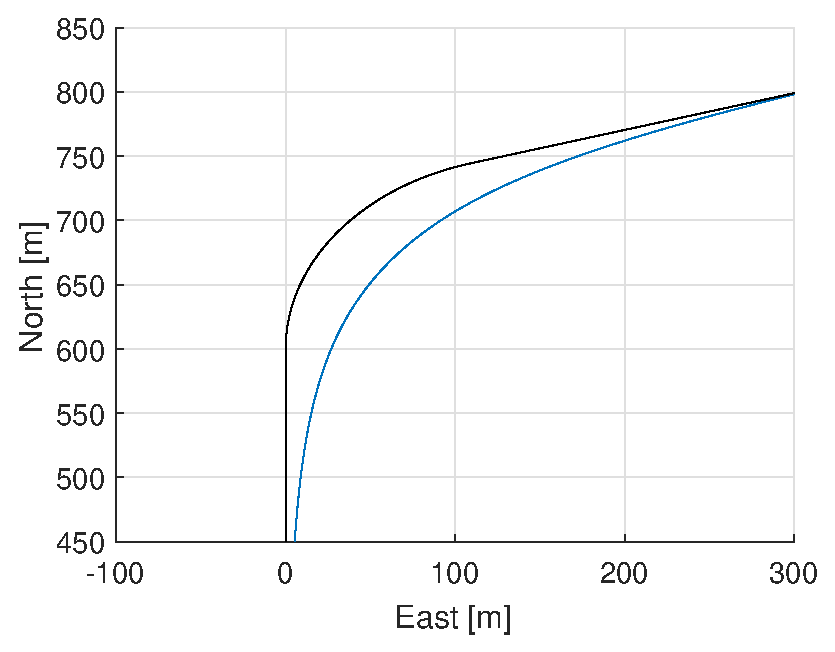
\includegraphics[width=0.5\textwidth, keepaspectratio=true]{../../results/opt/turns/curved/fig_70deg/uav_position.eps}}
	\qquad
	\subfloat[Camera position][Camera poistion.]{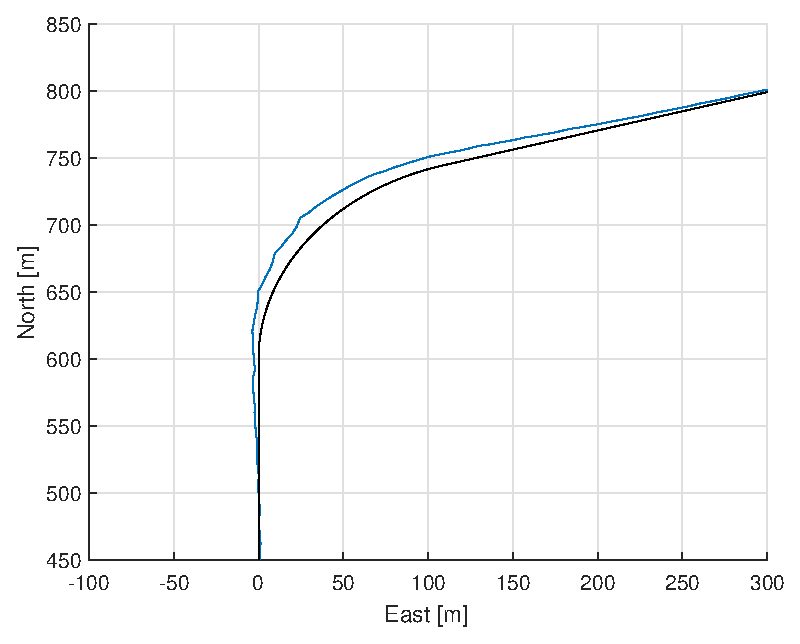
\includegraphics[width=0.5\textwidth, keepaspectratio=true]{../../results/opt/turns/curved/fig_70deg/camera_position.eps}}}
    \makebox[\textwidth][c]{
	\subfloat[Attitude angles]{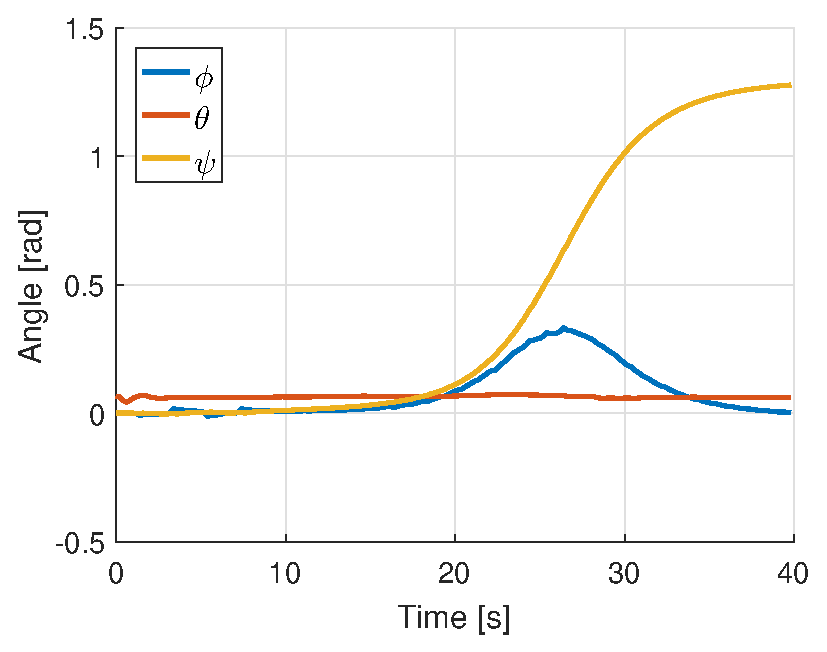
\includegraphics[width=0.5\textwidth, keepaspectratio=true]{../../results/opt/turns/curved/fig_70deg/attitude.eps}}
	\qquad
	\subfloat[Altitude]{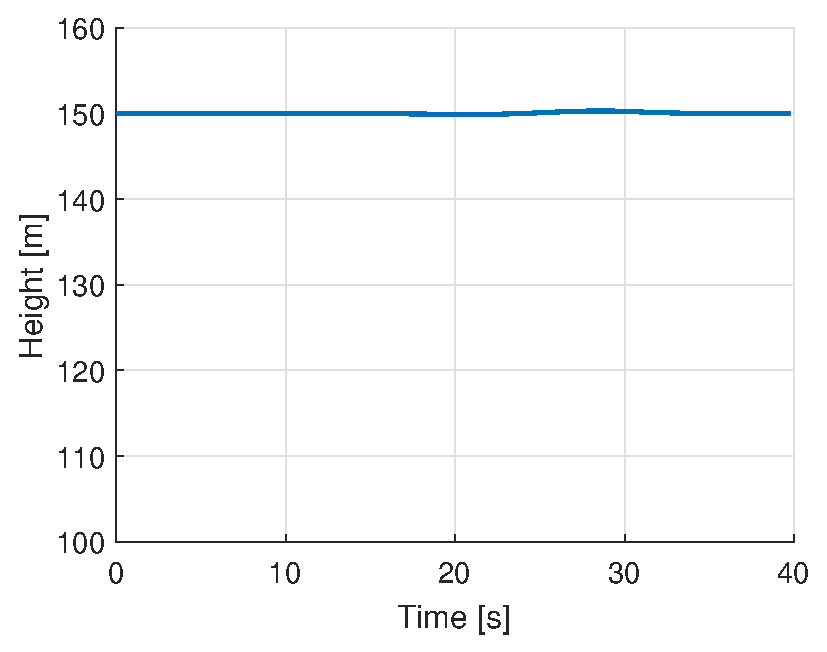
\includegraphics[width=0.5\textwidth, keepaspectratio=true]{../../results/opt/turns/curved/fig_70deg/height.eps}}}
	\caption{Results of optimizing a curved $70\degree$ turn.}
	\label{fig:turns_cur_70deg_pos}
\end{figure}


\subsubsection{Linear $70\degree$ Turn}

Optimizing a path containing a $70\degree$ linear turn returns a very different result than for the curved turn. As can be seen in Figure \ref{fig:turns_lin_70deg_pos1}, the MPC is not able to achieve stable flight throughout the turn, and it is difficult to point to one exact reason for why the optimization fails. The aircraft is about halfway through the turn when it suddenly banks to the left and enters a spiral. This could be for the same reason as when the horizon length is too short, that it tries to cover the path by moving the camera position using roll. It is also possible that the optimization algorithm could not find a feasible solution. When it cannot find a feasible solution it still returns some values and tries to continue, but in most cases the system is already unstable at this point, so it is not able to get it back to a stable state.

\begin{figure}
	\makebox[\textwidth][c]{
	\subfloat[UAV position][UAV position.]{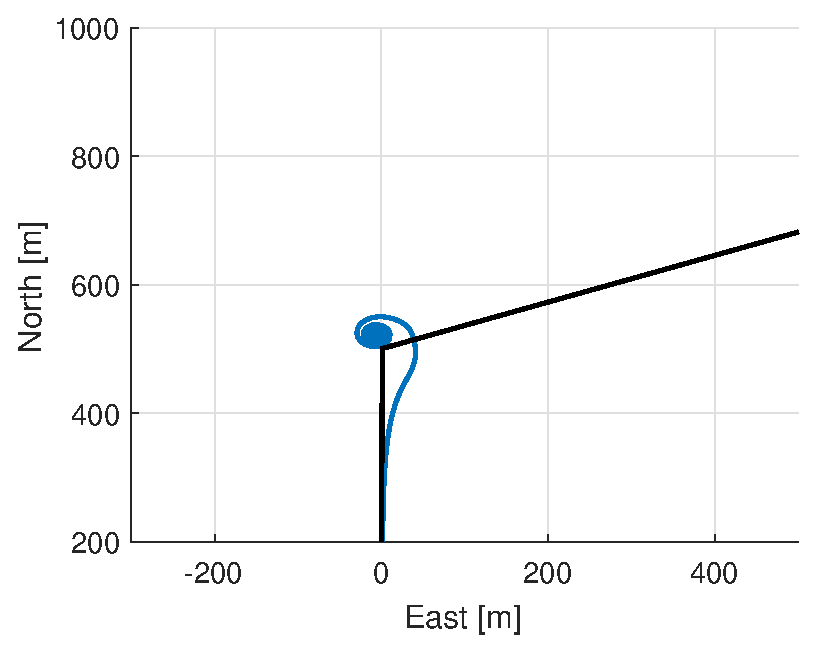
\includegraphics[width=0.5\textwidth, keepaspectratio=true]{../../results/opt/turns/linear/fig_70deg/uav_position_1.eps}}
	\qquad
	\subfloat[Camera position][Camera poistion.]{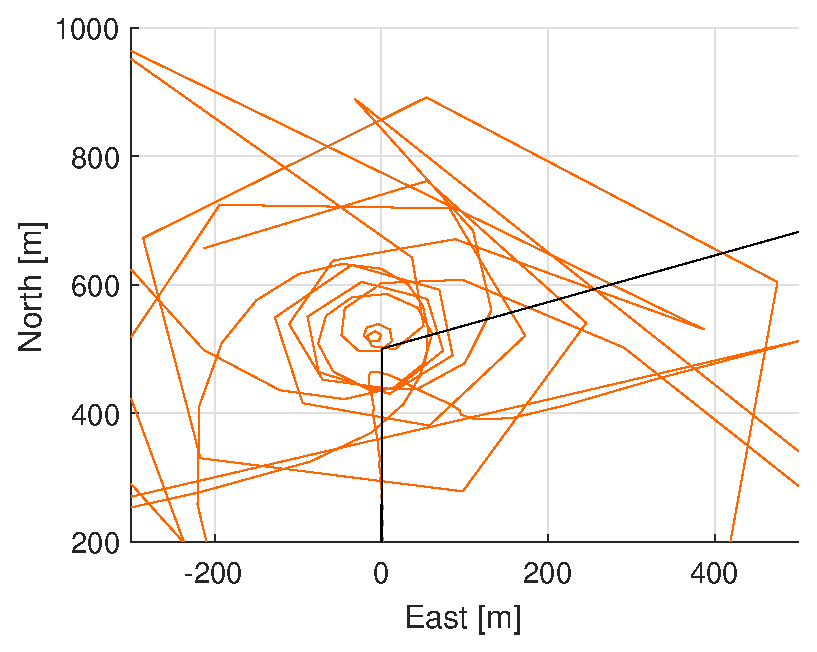
\includegraphics[width=0.5\textwidth, keepaspectratio=true]{../../results/opt/turns/linear/fig_70deg/camera_position_1.eps}}}
	\makebox[\textwidth][c]{
	\subfloat[Attitude angles]{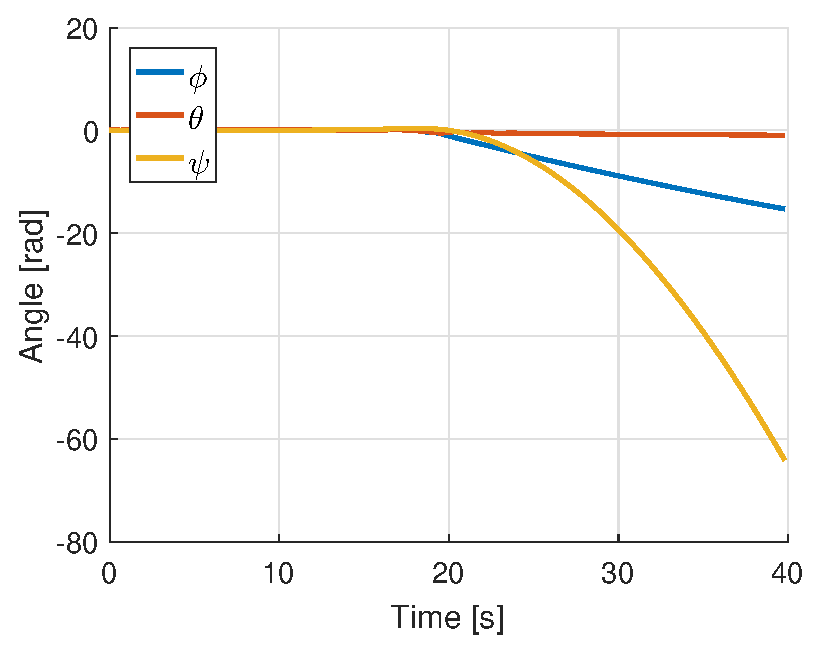
\includegraphics[width=0.5\textwidth, keepaspectratio=true]{../../results/opt/turns/linear/fig_70deg/attitude_1.eps}}
	\qquad
	\subfloat[Altitude]{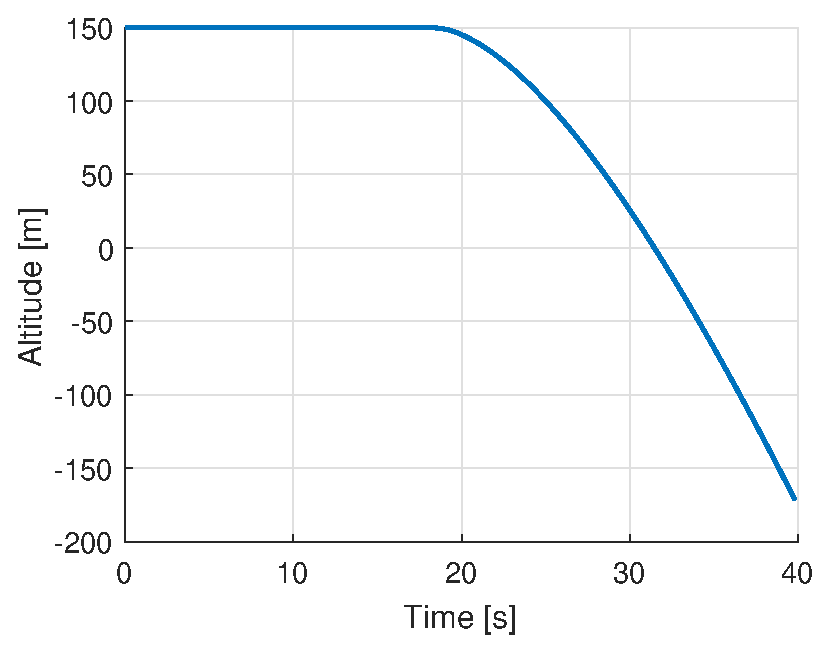
\includegraphics[width=0.5\textwidth, keepaspectratio=true]{../../results/opt/turns/linear/fig_70deg/height_1.eps}}}
	\caption{Results of optimizing a linear $70\degree$ turn with $10^{-1}$ weight on camera position.}
	\label{fig:turns_lin_70deg_pos1}
\end{figure}

In an attempt to achieve stable optimization of the corner, the weighting of the camera position in the objective function was reduced. The result of changing the weighting from $10^{-1}$ to $10^{-3}$ can be seen in Figure \ref{fig:turns_lin_70deg_pos3}. This tuning results in a stable flight, but the path tracking is not as precise and smooth as for the $45\degree$ turn. In addition the resulting camera path consists of several loops. This occurs as a combination of both the roll angle and pitch angle changing at the same time.

\begin{figure}
	\makebox[\textwidth][c]{
	\subfloat[UAV position][UAV position.]{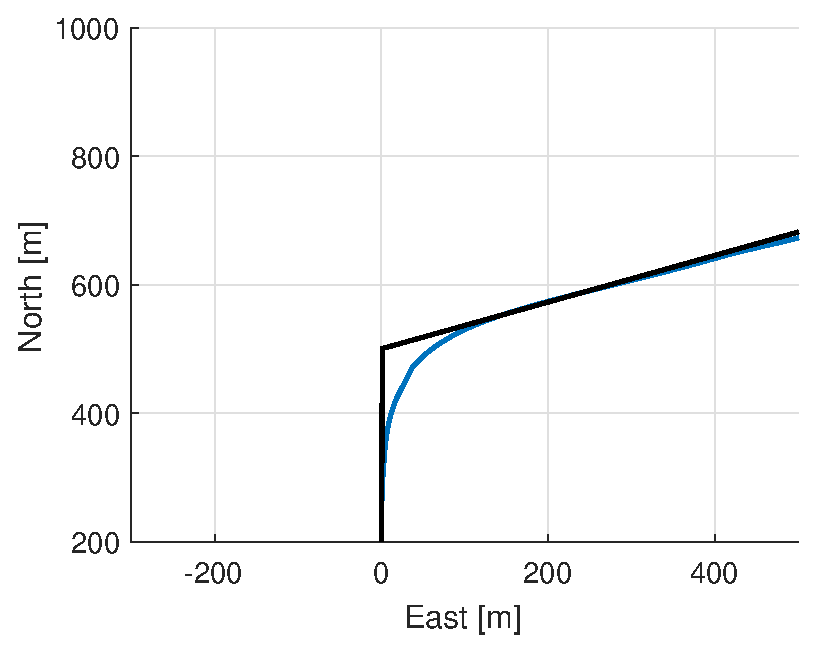
\includegraphics[width=0.5\textwidth, keepaspectratio=true]{../../results/opt/turns/linear/fig_70deg/uav_position_3.eps}}
	\qquad
	\subfloat[Camera position][Camera poistion.]{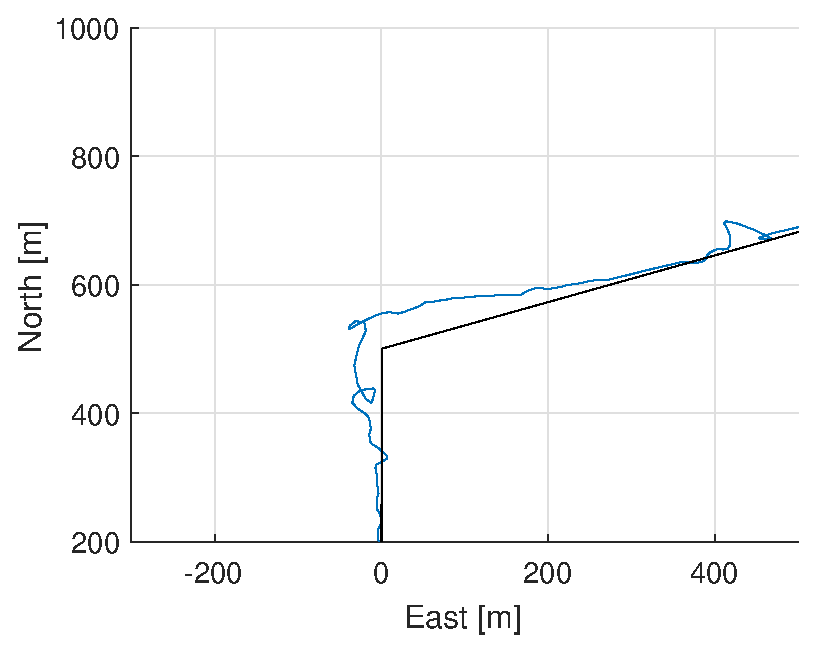
\includegraphics[width=0.5\textwidth, keepaspectratio=true]{../../results/opt/turns/linear/fig_70deg/camera_position_3.eps}}}
	\makebox[\textwidth][c]{
	\subfloat[Attitude angles]{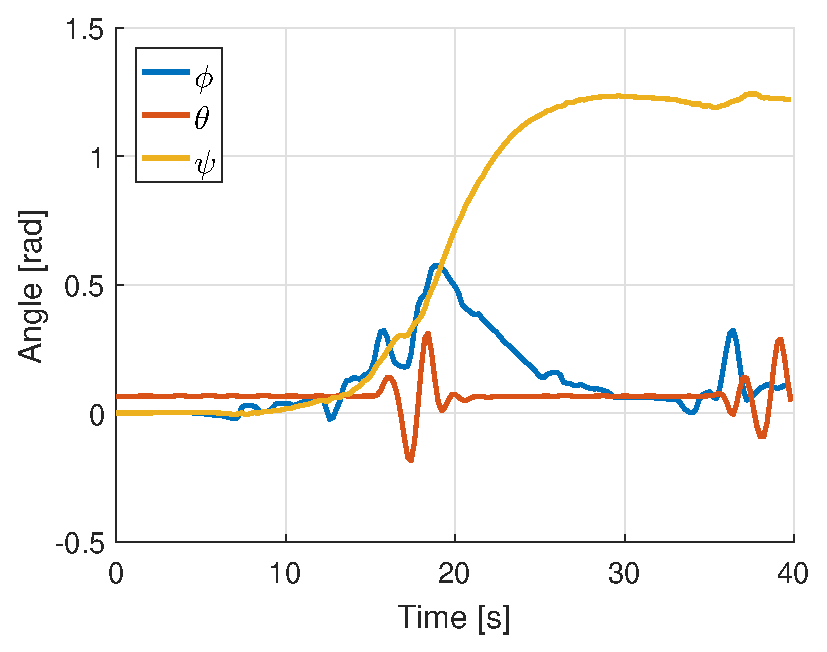
\includegraphics[width=0.5\textwidth, keepaspectratio=true]{../../results/opt/turns/linear/fig_70deg/attitude_3.eps}}
	\qquad
	\subfloat[Altitude]{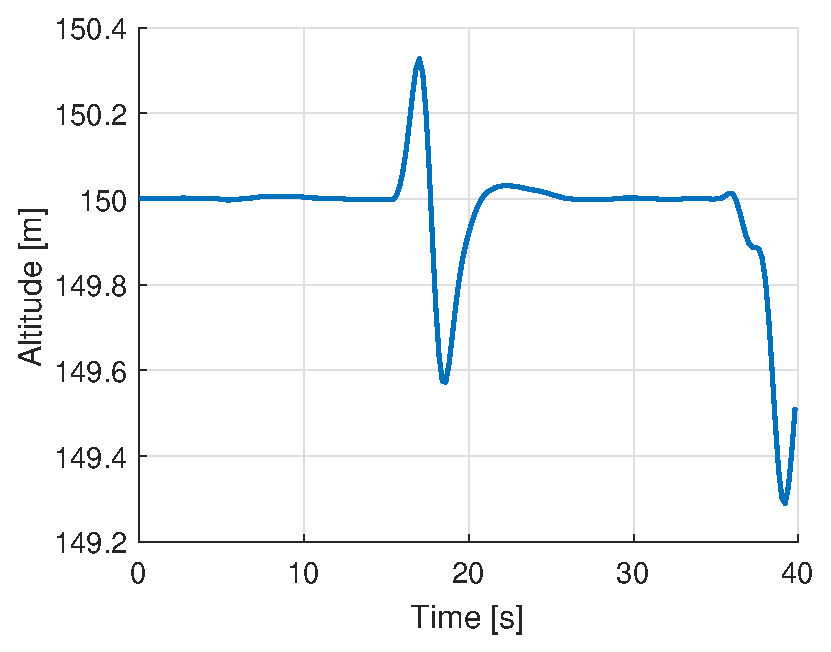
\includegraphics[width=0.5\textwidth, keepaspectratio=true]{../../results/opt/turns/linear/fig_70deg/height_3.eps}}}
	\caption{Results of optimizing a linear $70\degree$ turn with $10^{-3}$ weight on camera position.}
	\label{fig:turns_lin_70deg_pos3}
\end{figure}

A third attempt on a linear $70\degree$ turn was made, this time with a weighting of the camera position of $10^{-5}$. As can be seen in Figure \ref{fig:turns_lin_70deg_pos5} this results in a stable flight. The path tracking on the other hand, is poor. With this tuning the weight on the camera position is so much lower than on the other states included in the objective function, so that the path with the lowest cost is not the path that tracks the ground path.

\begin{figure}
	\makebox[\textwidth][c]{
	\subfloat[UAV position][UAV position.]{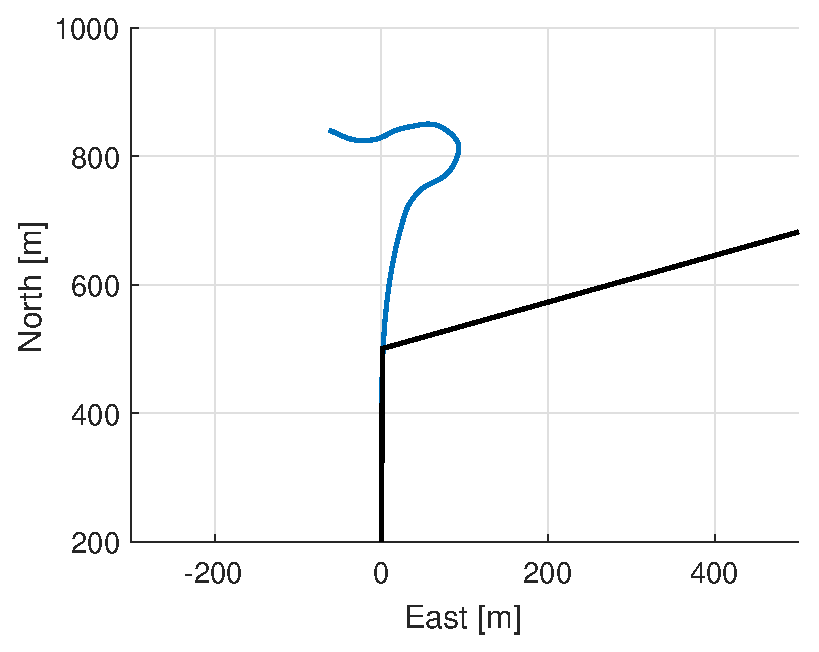
\includegraphics[width=0.5\textwidth, keepaspectratio=true]{../../results/opt/turns/linear/fig_70deg/uav_position_5.eps}}
	\qquad
	\subfloat[Camera position][Camera poistion.]{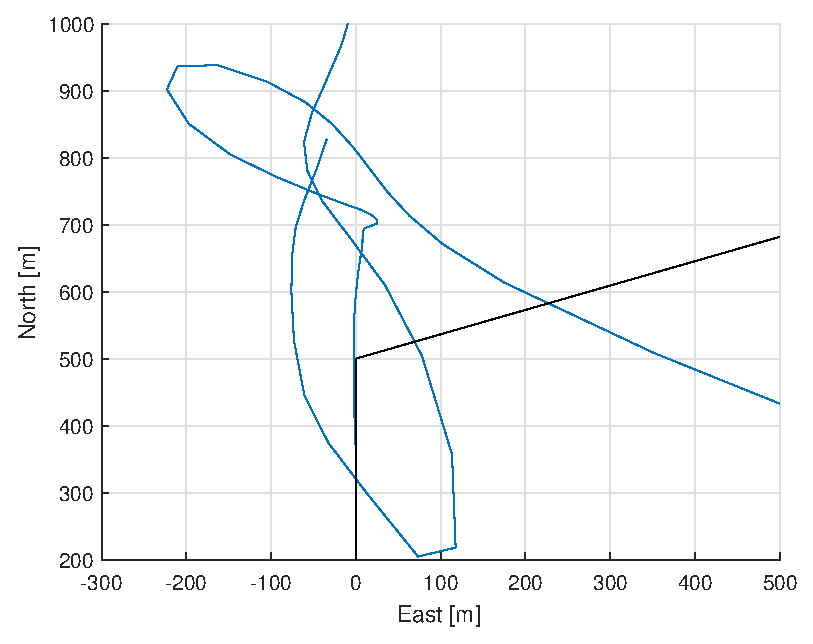
\includegraphics[width=0.5\textwidth, keepaspectratio=true]{../../results/opt/turns/linear/fig_70deg/camera_position_5.eps}}}
	\makebox[\textwidth][c]{
	\subfloat[Attitude angles]{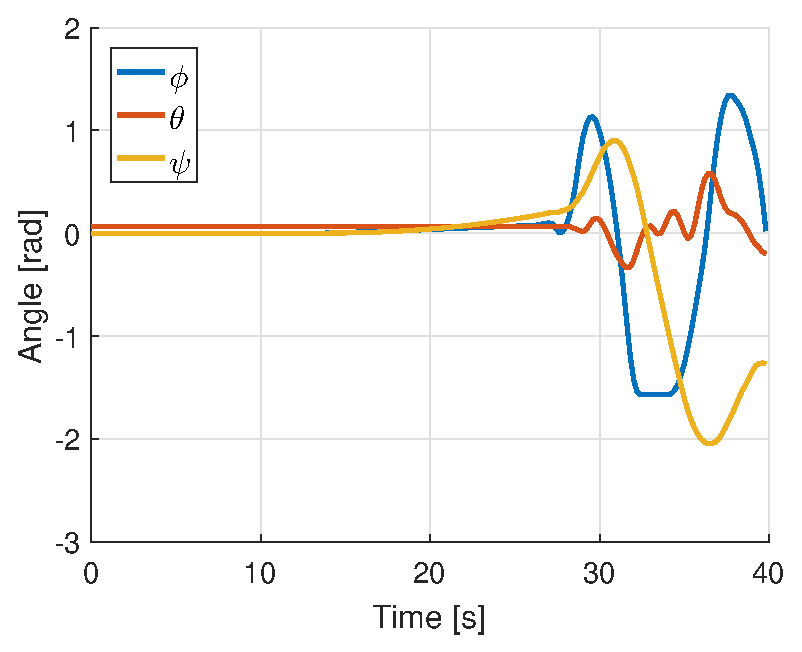
\includegraphics[width=0.5\textwidth, keepaspectratio=true]{../../results/opt/turns/linear/fig_70deg/attitude_5.eps}}
	\qquad
	\subfloat[Altitude]{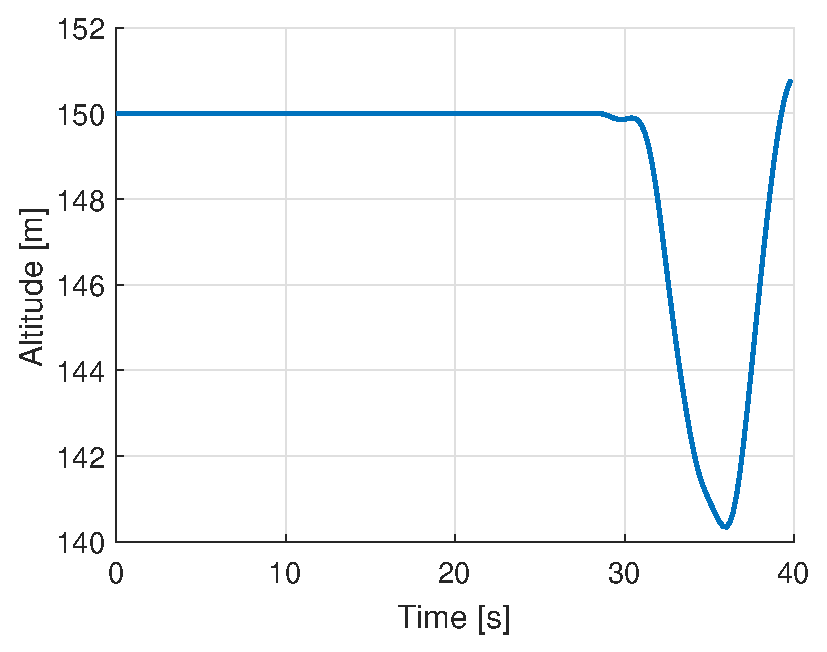
\includegraphics[width=0.5\textwidth, keepaspectratio=true]{../../results/opt/turns/linear/fig_70deg/height_5.eps}}}
	\caption{Results of optimizing a linear $70\degree$ turn with $10^{-5}$ weight on camera position.}
	\label{fig:turns_lin_70deg_pos5}
\end{figure}